\chapter{Implementation}

\section{Directory Structure}
The directory structure (for the application only) is defined as follows:

\begin{itemize}
    \item \textbf{app} contains various Laravel application components, such as models, controllers, and policies
    \item \textbf{bootstrap} Framework code used by Laravel to bootstrap the application
    \item \textbf{config} Framework code that define configurations for various Laravel utilities and functionalities
    \item \textbf{database} Database factories, migration definitions, and seeding tools are in this directory.
    \item \textbf{docs} Documentation generated by Sami is stored here. This is explored in more detail in Chapter 7.
    \item \textbf{node\_modules} This contains Node.js dependencies installed by Laravel Mix and are used in development. This is discussed in greater detail in Chapter 7.
    \item \textbf{public} is the front-facing directory containing the application entry-point, as well as compiled assets and images used for social media.
    \item \textbf{routes} HTTP Application routes are defined in the files contain within this directory.
    \item \textbf{resources} Views written in Laravel Blade are kept in this folder, along with stylesheets and scripts that comprise the front-end.
    \item \textbf{storage} Laravel stores log files here, and generated PDF files for download are kept here. A cache for quick loading is also stored here.
    \item \textbf{tests} PHPUnit tests are kept here, and are covered in Chapter 6.
    \item \textbf{vendor} Similar to \textit{node\_modules}, this folder stores PHP dependencies used by Laravel, as well as additional third-party libraries.
\end{itemize} \cite{W3Schools1}

\section{Method of Action}
The Laravel developers acknowledge that having a basic, high-level understanding of how a framework works is important for not only having a basic grasp of how the application works, but also to make 'everything feel less magical'. \cite{Laravel6} This is important as frameworks are characterised by carrying out substantial amounts of work for you, in order to drastically reduce development time and to produce better quality applications, and are generally recommended by the greater web development community. \cite{Mozilla3}

\begin{figure}[!ht]
    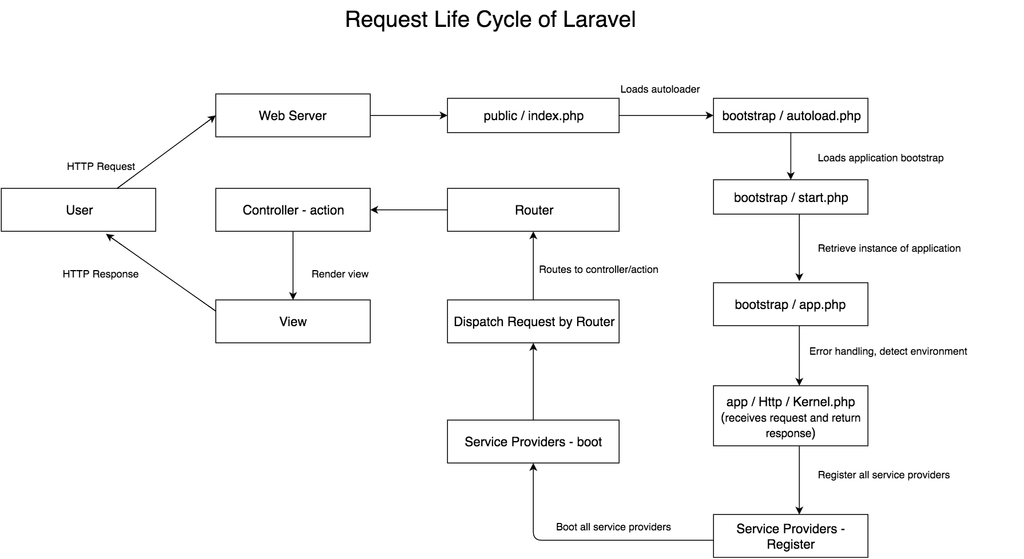
\includegraphics[width=1.0\textwidth]{Figures/laravel-request}
    \caption{Diagram that shows how the Request Lifecycle for the Laravel framework operates.}
    \label{fig:laravel-requests} \cite{Mallow1}
\end{figure}

When a HTTP (Hypertext Transfer Protocol) request is received by the web server by navigating to the \textbf{index.php} file in the \textit{public} directory, the application is quickly bootstrapped, loading all necessary libraries and components by means of the PSR-4 autoload file, which is a widely accepted PHP coding standard and was generated by Composer, the PHP package manager when the application was first installed. \cite{PSR1} From here, the application can determine how to 'route' the request based on route definitions and the URL (Uniform Resource Locator) path, delegating actions to the appropriate controllers and their models defined in those definitions, before passing data to a view, and returning it to the user. \cite{Laravel6} According to Stauffer, Laravel's approach 'brings your ideas to reality with no wasted code' and 'modern programming standards.' \cite{LaravelUp1}

\section{HTTP Routes}



\section{Models and Relationships}

\section{Users}

\subsection{Authentication}

\subsection{Authorisation and Policies}

\section{Role Types}

\section{Role Competencies}

\section{Roles}

\section{Locations}

\section{Locomotives}

\section{Operations and Shifts}

\section{Calendar View}

\section{PDF Export Functionality}

\section{Administration Panel}

\section{Additional Webpages}